\documentclass{article}
\usepackage[utf8]{inputenc}
\usepackage{amsmath}
\usepackage{graphicx}
\usepackage{subcaption}
\usepackage{float}
\usepackage{geometry}
\geometry{a4paper, margin=1in}

\title{SH1017 Physics for Engineering Mathematics Lab 2}
\author{Lucas Frykman}
\date{\today}

\begin{document}

\maketitle

% \section*{Background}
% This report details the findings from Computer Lab 2, focusing on the simulation of wave interference and diffraction using point sources. We investigate the behavior of interference patterns as we vary source configurations, slit widths, and distances. The electric field $E(\mathbf{r}, t)$ from $N$ identical sources at positions $\mathbf{r}_i$ is given by the superposition:
% \begin{equation}
% E(\mathbf{r}, t) = \sum_{i=1}^{N} \frac{A}{|\mathbf{r} - \mathbf{r}_i|} \cos(k|\mathbf{r} - \mathbf{r}_i| - \omega t)
% \end{equation}
% The time-averaged intensity measured on a detector screen at distance $D$ is:
% \begin{equation}
% \overline{E^2} = \frac{|A|^2}{r^2} \left( \frac{N}{2} + \sum_{i=1}^{N-1} \sum_{j=i+1}^N \cos(k|\mathbf{r} - \mathbf{r}_i| - k|\mathbf{r} - \mathbf{r}_j|) \right)
% \end{equation}

\section*{Q1: Interference from Point Sources}

\textbf{Method:} Using \texttt{interference.py}, we simulate two coherent point sources and observe how the interference pattern changes with the separation distance $d$ and by adding a third source.

\begin{figure}[H]
    \centering
    \begin{subfigure}[b]{0.45\textwidth}
        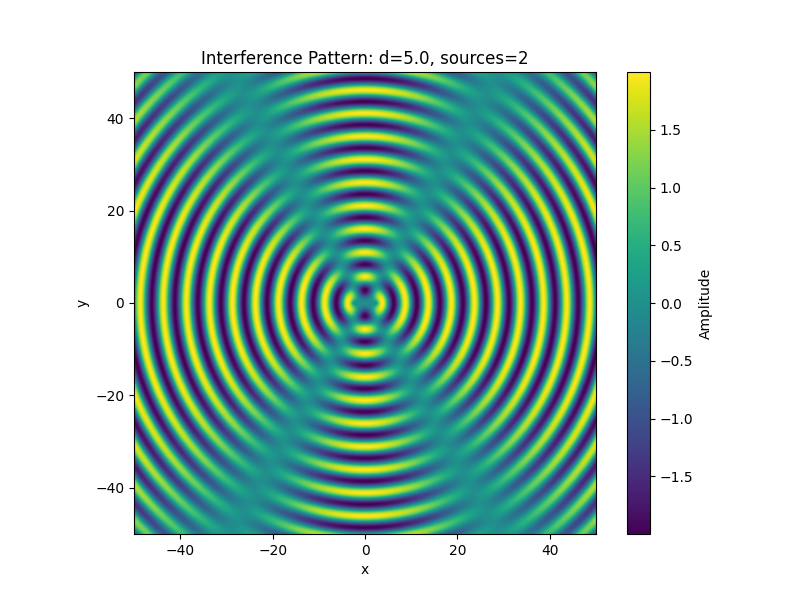
\includegraphics[width=\textwidth]{figures/p1_d10.png}
        \caption{$d=5$}
    \end{subfigure}
    \begin{subfigure}[b]{0.45\textwidth}
        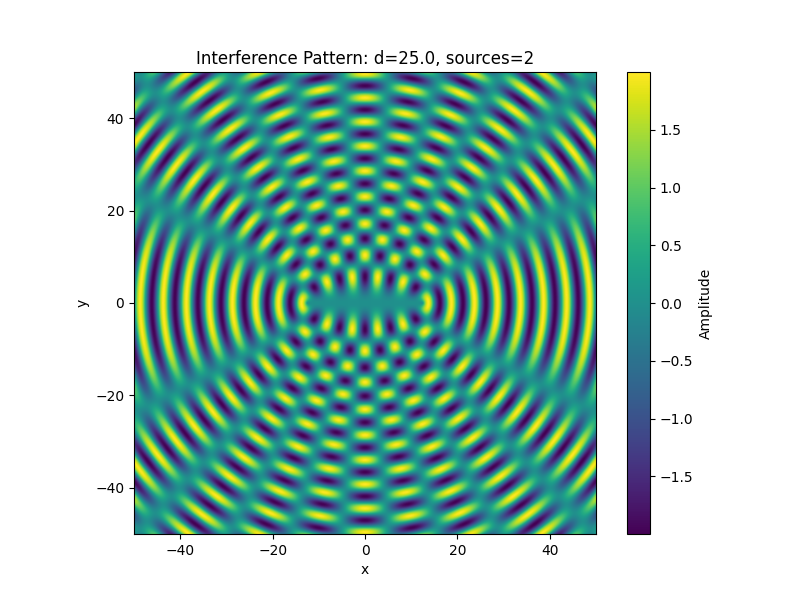
\includegraphics[width=\textwidth]{figures/p1_d20.png}
        \caption{$d=25$}
    \end{subfigure}
    \begin{subfigure}[b]{0.45\textwidth}
        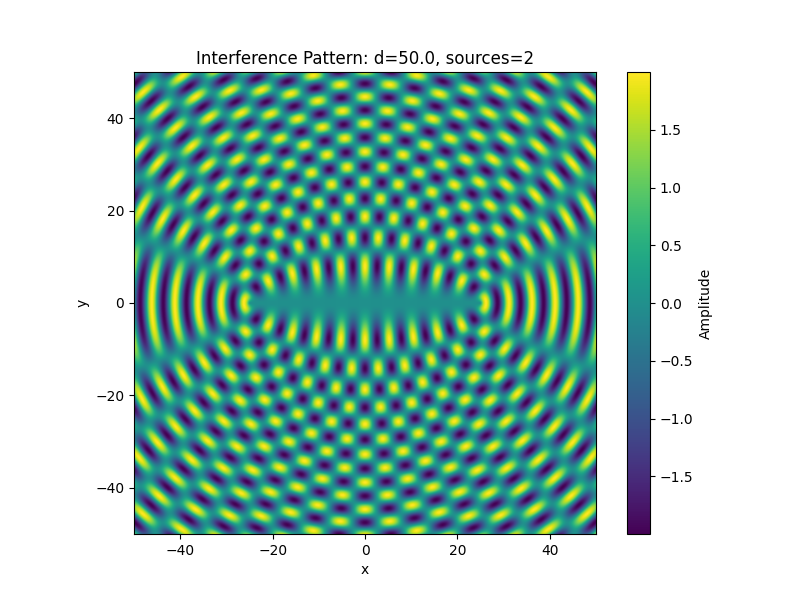
\includegraphics[width=\textwidth]{figures/p1_d40.png}
        \caption{$d=50$}
    \end{subfigure}
    \begin{subfigure}[b]{0.45\textwidth}
        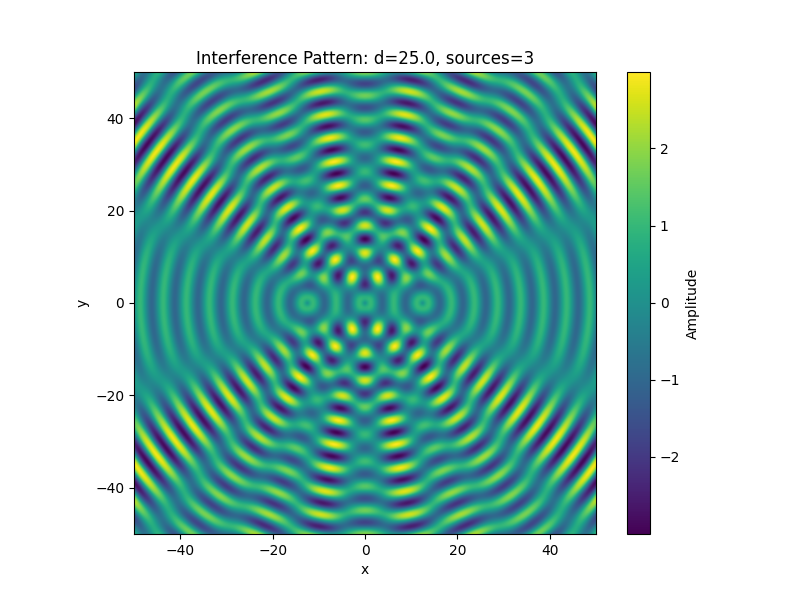
\includegraphics[width=\textwidth]{figures/p1_3sources.png}
        \caption{3 sources, $d=25$}
    \end{subfigure}
    \caption{Interference patterns for different configurations ($\lambda=5.0$ mm, $100 \times 100$ mm area).}
    \label{fig:p1}
\end{figure}

% \textbf{Theory:} According to $N$-slit interference theory, increasing the distance $d$ between sources should decrease the angular separation between fringes, leading to more fringes within a given area. Adding more sources 
% should sharpen the primary maxima and introduce more smaller maxima between them.

\textbf{Results:} As seen in Figure \ref{fig:p1}, increasing the distance $d$ between the 
sources increases the number of interference fringes (maxima and minima) within the same area which corresponds to a smaller angular separation. Adding a third source between the two existing ones 
sharpens the primary maxima and introduces several more smaller maxima between them. 

\section*{Q2: Double Slit Interference}

\textbf{Method:} Using the code from \texttt{doubleslit.py}, we simulate the interference pattern on a screen at distance $D$ from two slits separated by $d$, 
using $\lambda = 500$ nm. 

\begin{figure}[H]
    \centering
    \begin{subfigure}[b]{0.8\textwidth}
        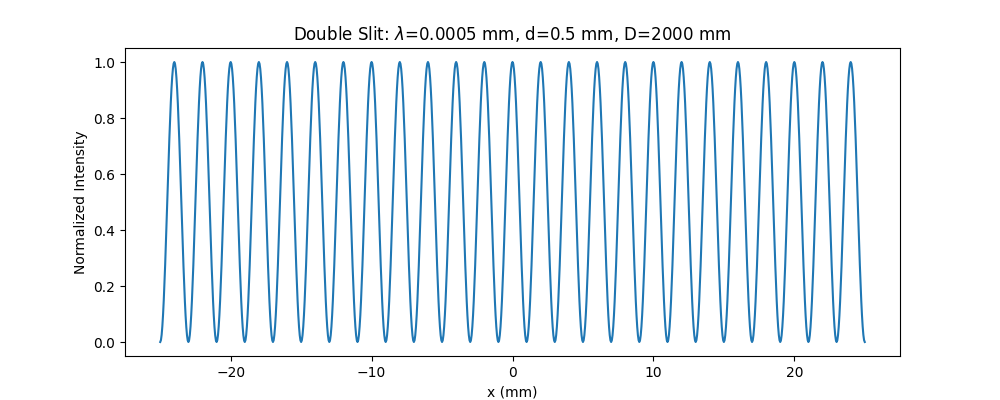
\includegraphics[width=\textwidth]{figures/p2_base.png}
        \caption{Base: $\lambda=0.0005$ mm, $d=0.5$ mm, $D=2000$ mm}
    \end{subfigure}
    \begin{subfigure}[b]{0.8\textwidth}
        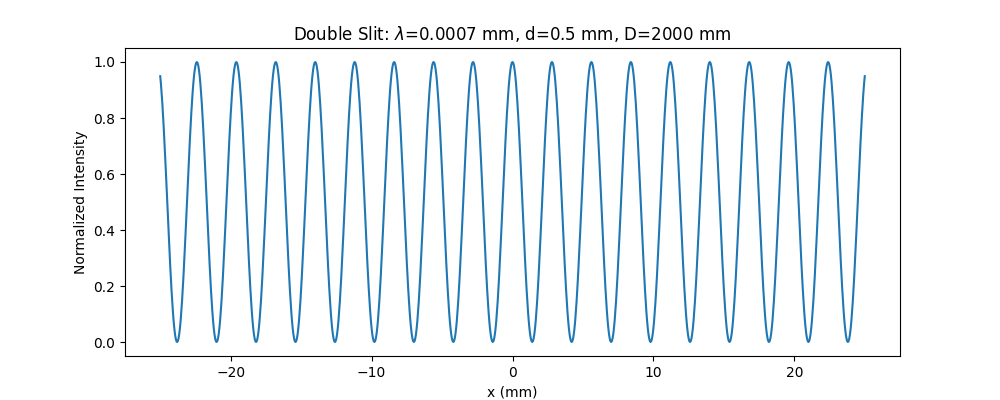
\includegraphics[width=\textwidth]{figures/p2_lambda_red.png}
        \caption{Larger $\lambda$: $\lambda=0.0007$ mm, $d=0.5$ mm, $D=2000$ mm}
    \end{subfigure}
    \begin{subfigure}[b]{0.7\textwidth}
        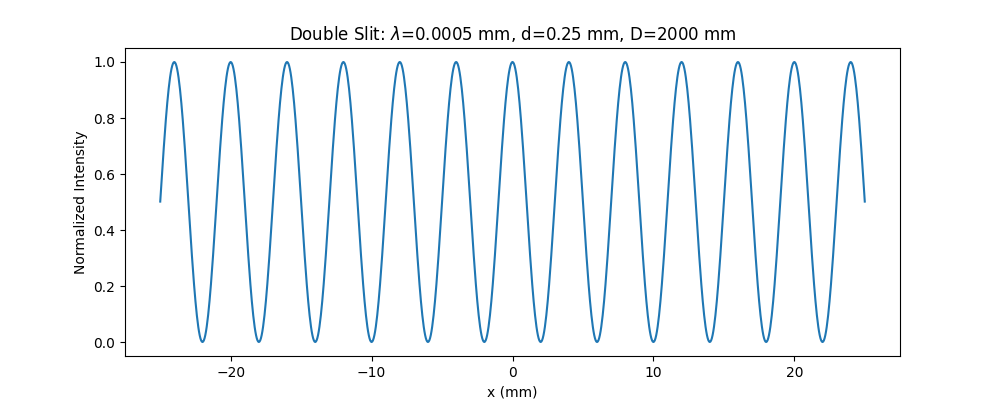
\includegraphics[width=\textwidth]{figures/p2_d_small.png}
        \caption{Smaller $d$: $\lambda=0.0005$ mm, $d=0.25$ mm, $D=2000$ mm}
    \end{subfigure}
    \begin{subfigure}[b]{0.8\textwidth}
        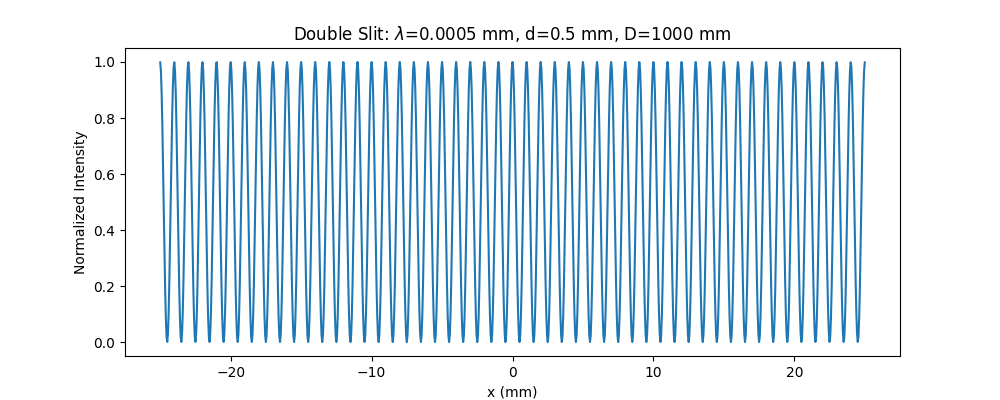
\includegraphics[width=\textwidth]{figures/p2_bigd_small.png}
        \caption{Smaller $D$: $\lambda=0.0005$ mm, $d=0.5$ mm, $D=1000$ mm}
    \end{subfigure}
    \label{fig:p2}  
\end{figure}

\textbf{Theory:} The distance between maxima is given by $\Delta x = \lambda D / d$ where $\lambda$ is the wavelength, $D$ is the distance to the screen, and $d$ is the distance between the slits. 
% Without these approximations, the exact geometric distance $r = \sqrt{D^2 + x^2}$ must be considered, 
% meaning the distance between fringes on a flat screen should 
% increase as we move further from the center compared to what 
% the simple formula predicts.

\textbf{Results:} The results for various parameters are summarized below:
\begin{table}[h]
\centering
\begin{tabular}{|l|c|c|c|c|c|}
\hline
Case & $\lambda$ (mm) & $d$ (mm) & $D$ (mm) & Theoretical $\Delta x$ (mm) & Measured $\Delta x$ (mm) \\ \hline
Base & 0.0005 & 0.5 & 2000 & 2.0000 & 2.0000 \\
Larger $\lambda$ & 0.0007 & 0.5 & 2000 & 2.8000 & 2.8000 \\
Smaller $d$ & 0.0005 & 0.25 & 2000 & 4.0000 & 4.0000 \\
Smaller $D$ & 0.0005 & 0.5 & 1000 & 1.0000 & 1.0000 \\
\hline
\end{tabular}

\caption{Comparison of theoretical and measured fringe spacing.}
\label{tab:p2}
\end{table}

The numerical approximation of $\Delta x$ is accurate to the theoretical value within 4 sig figs. And as expected (see figure 2 and table 1)
the distance betwen maxima increases linearly with both distance to the screen and wavelength and it decreases with distance between the slits.

% The measured values differ and are consistently larger than the 
% simple formula $\Delta x = \lambda D / d$. This is because the 
% formula assumes a small-angle approximation ($\sin \theta \approx \theta$) 
% and a planar detector screen, whereas the simulation uses the exact geometric 
% distance $r = \sqrt{D^2 + x^2}$. As $x$ increases, the distance between fringes 
% on a flat screen increases compared to an arc. This geometric effect accounts 
% for the observed deviations from the theoretical approximation.

\section*{Q3: Single Slit Model}

\textbf{Method:} We modify \texttt{doubleslit.py} to approximate a single slit of width $w = 0.05$ mm by placing $N \in \{2, 3, 5, 10\}$ point sources along the slit, using $\lambda = 0.0005$ mm and $D=2000$ mm. We investigate how the peak intensity and width depend on $N$ and $w$.

\begin{figure}[H]
    \centering
    \begin{subfigure}[b]{0.45\textwidth}
        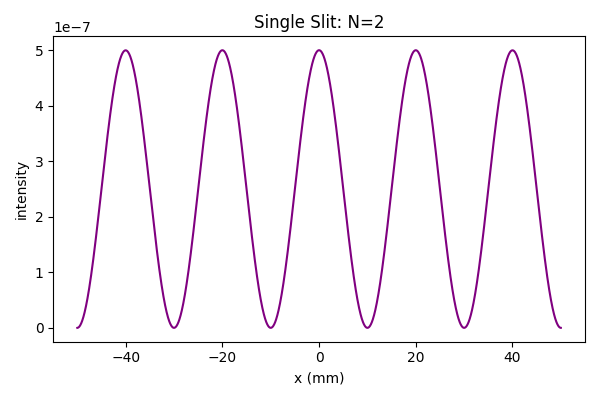
\includegraphics[width=\textwidth]{figures/p3_N2.png}
        \caption{$N=2$}
    \end{subfigure}
    \begin{subfigure}[b]{0.45\textwidth}
        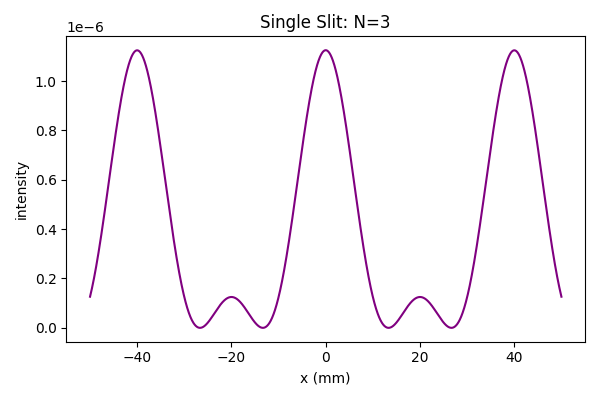
\includegraphics[width=\textwidth]{figures/p3_N3.png}
        \caption{$N=3$}
    \end{subfigure}
    \begin{subfigure}[b]{0.45\textwidth}
        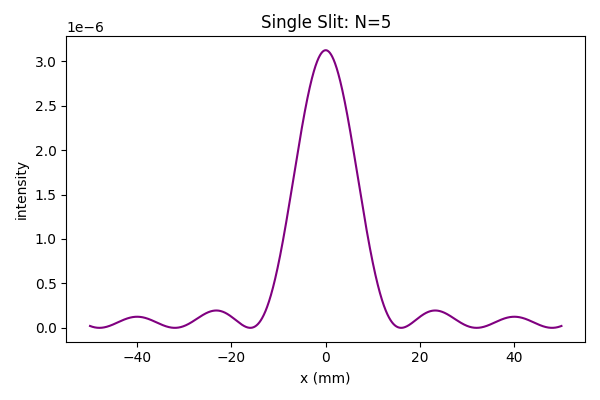
\includegraphics[width=\textwidth]{figures/p3_N5.png}
        \caption{$N=5$}
    \end{subfigure}
    \begin{subfigure}[b]{0.45\textwidth}
        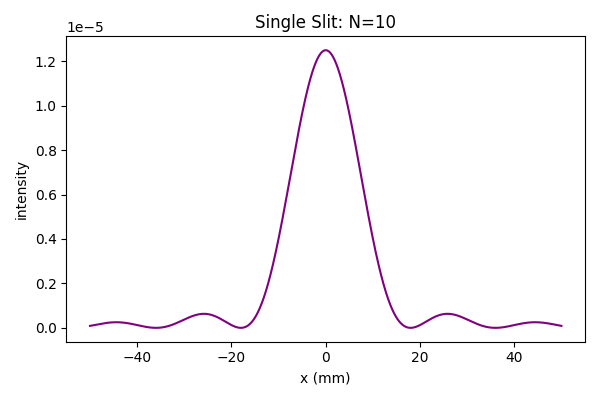
\includegraphics[width=\textwidth]{figures/p3_N10.png}
        \caption{$N=10$}
    \end{subfigure}
    \caption{Intensity distribution for a single slit modeled with varying $N$ sources (\textbf{w=0.05} mm, $\lambda=0.0005$ mm, $D=2000$ mm).}
    \label{fig:p3_N}
\end{figure}

\begin{figure}[H]
    \centering
    \begin{subfigure}[b]{0.45\textwidth}
        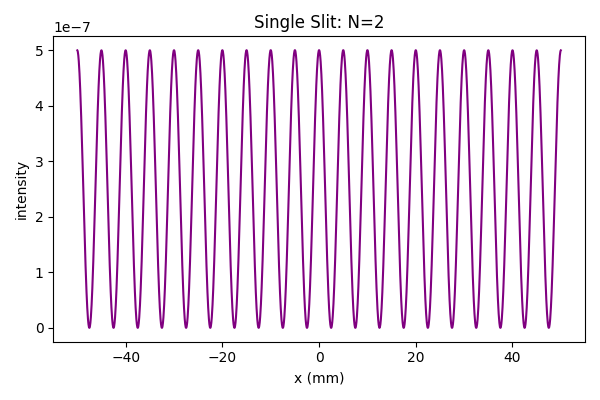
\includegraphics[width=\textwidth]{figures/p3_N_diff_w2.png}
        \caption{$N=2$}
    \end{subfigure}
    \begin{subfigure}[b]{0.45\textwidth}
        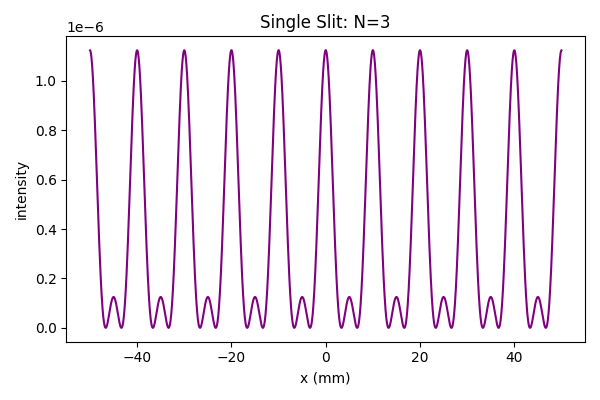
\includegraphics[width=\textwidth]{figures/p3_N_diff_w3.png}
        \caption{$N=3$}
    \end{subfigure}
    \begin{subfigure}[b]{0.45\textwidth}
        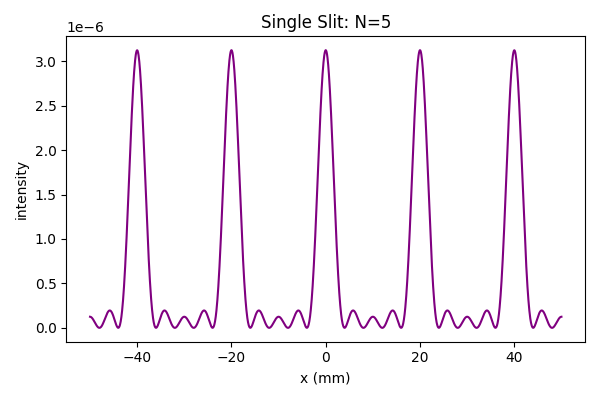
\includegraphics[width=\textwidth]{figures/p3_N_diff_w5.png}
        \caption{$N=5$}
    \end{subfigure}
    \begin{subfigure}[b]{0.45\textwidth}
        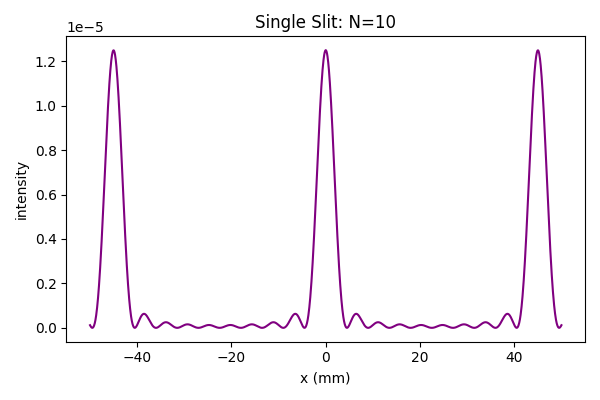
\includegraphics[width=\textwidth]{figures/p3_N_diff_w10.png}
        \caption{$N=10$}
    \end{subfigure}
    \caption{Intensity distribution for a single slit modeled with varying $N$ sources (\textbf{w=0.2} mm, $\lambda=0.0005$ mm, $D=2000$ mm).}
    \label{fig:p3_w}
\end{figure}

% \textbf{Theory:} We theorize that the width of the central maxima is inversely proportional to the slit width, according to $\theta \approx \lambda/w$. This implies that increasing the slit width will result in a narrower central maxima. We also expect that increasing the number of sources $N$ will yield a higher intensity peak.

\textbf{Results:} As seen in Figure \ref{fig:p3_N} ($w=0.05$ mm), we can observe that a greater $N$ implies a higher intensity peak. For example, for $N=2$ the peak is much lower than for $N=10$. We then varied $w$ as shown in Figure \ref{fig:p3_w}. The figures indicate that a smaller $w$ ($0.05$ mm) results in a wider peak where the central maxima dominates, while a greater $w$ ($0.2$ mm) results in narrower peaks that are packed more tightly together.
\newpage
\section*{Q4: Realistic Double Slit Model}

\textbf{Method:} We copied 2 of the "realistic" slits from problem 3 ($N=10$, $w=0.05$ mm) and separated them by $d=0.5$ mm and compared it to the point-source model.

\begin{figure}[H]
    \centering
        \begin{subfigure}[b]{\textwidth}
        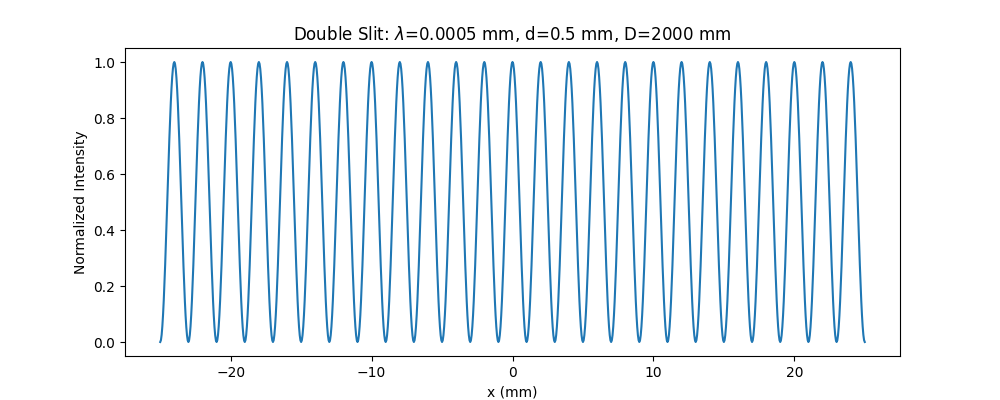
\includegraphics[width=\textwidth]{figures/p2_base.png}
        \caption{Point source model}
    \end{subfigure}
    \begin{subfigure}[b]{\textwidth}
        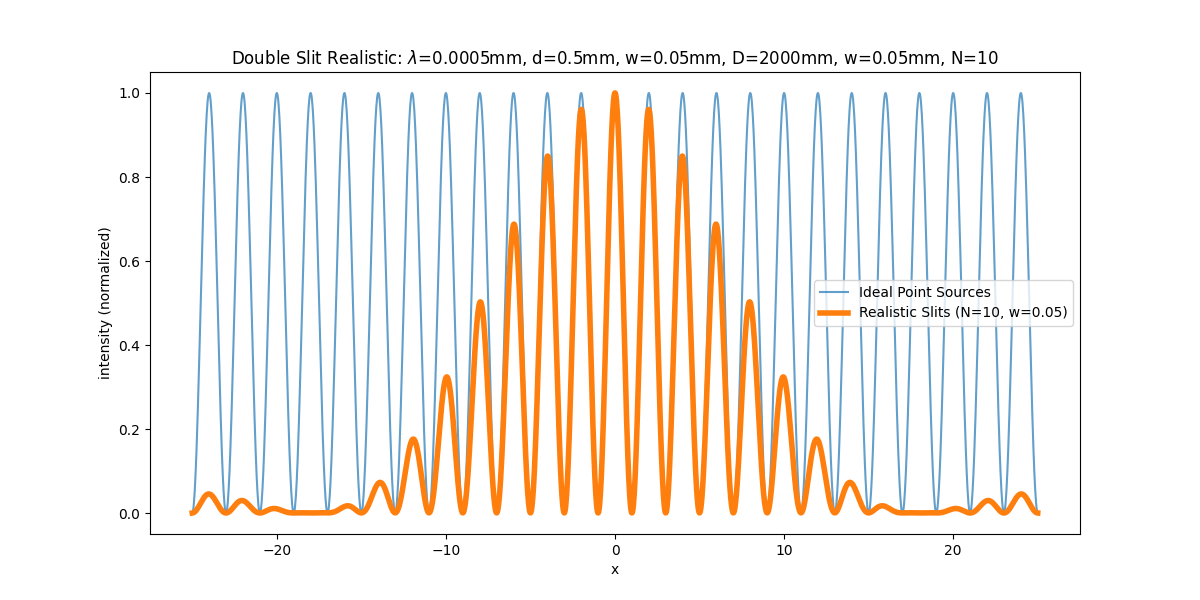
\includegraphics[width=\textwidth]{figures/p4_comparison.png}
        \caption{Realistic slit model}
    \end{subfigure}
    \caption{Comparison between point source double slit ($d=0.5$ mm, $\lambda=0.0005$ mm, $D=2000$ mm).} and realistic doubel slit (with discretization along a continous width $N=10$, $w=0.05$ mm), 
    \label{fig:p4}
\end{figure}

% \textbf{Theory:} A realistic double slit should show similar interference behavior to the ideal point sources, but with some effects from the single slit width we explored in Q3.

\textbf{Results:} What can be observed from the graphs in Figure \ref{fig:p4} is that they seem to agree on the whole. Both the point 
source model and the realistic model have similar distances between their peaks. The main difference is that the realistic model's peaks 
get smaller further from the center.

\end{document}
